\section{Evaluation in the energy norm}\label{sec:checks}

The norm of the loss decides what a network learns; the norm of the metric decides how
networks are compared. This section shows that the displacement error ranked the networks
opposite to their stress errors, and tests the two checks of \cref{sec:theory:detector},
which need no solution.

\subsection{Ranking by displacement and by stress}\label{sec:checks:ranking}

\begin{figure}[tbp]
\centering
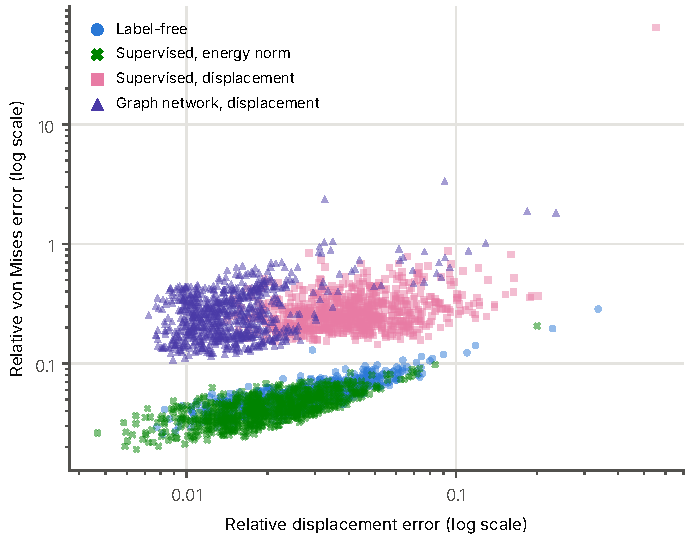
\includegraphics[width=0.72\linewidth]{generated/fig_disp_vs_stress.pdf}
\caption{Three dimensions, networks trained on 1,024 instances: relative von Mises error against
relative displacement error for every validation instance and seed (\numThreePairs{} points
per network). The two networks trained in the energy norm, with and without the solutions,
lie at the bottom; the two trained on the displacement error lie higher, whatever their
displacement error. The graph network's points lie to the left of the label-free
transformer's, at lower displacement error, and above them, at higher von Mises error. The
point at the top right is instance No.~\numWorstIndex{} in seed \numThreeLabWorstSeed{}
(\cref{sec:norm:three}).}
\label{fig:reverse}
\end{figure}

The graph network, trained on the solutions with the displacement error, had the lowest mean
displacement error of the three-dimensional networks, \numThreeMgnDisp{},
\numThreeFreeOverMgnDisp{} times lower than the label-free transformer's (\cref{tab:3d}),
and the label-free transformer was the more accurate on every other metric. The reversal
held on most instances individually (\cref{fig:reverse}). Compared within each seed, the
graph network's displacement error was the lower on \numMgnDispLowerMin{} to
\numMgnDispLowerMax{} of the instances, but its von Mises error was the higher on
\numMgnVmHigher{} of the \numThreePairs{} instance-seed pairs, with a mean
\numThreeMgnOverFreeVm{} times higher, and its relative energy gap was the higher on at
least \numMgnGapHigherMin{} of the instances in every seed. On \numMgnLowerDispHigherVm{}
pairs both held at once. The peak stress error, which compares a single value per load case,
followed the pattern less closely: the graph network's was the lower on
\numMgnPeakLowerMin{} to \numMgnPeakLowerMax{} of the instances, although its mean was
\numThreeMgnOverFreePeak{} times higher. The relative energy gap thus ranked the two
networks as the von Mises error did, not as the displacement error did. In two dimensions
the graph network again had the lowest displacement error of the networks, \numCmMgnDisp{},
within the guard of the displacement-supervised transformer's, a von Mises error
\numCmMgnOverFreeVm{} times the label-free transformer's, and the largest relative energy
gap of the trained networks, \numCmMgnOverLabGap{} times the displacement-supervised
transformer's (\cref{tab:2d}). By \cref{rem:rank} such reversals are possible whenever the
displacement errors differ by a factor of less than $\kappa^{1/2}$, which on the instances
measured was at least about \numSqrtKappaMin{} (\cref{sec:methods:data}). These comparisons
use the solutions; for the predictions of one load case, differences of energy rank them
exactly as the relative energy gap does, without a solution (\cref{cor:rank}).

\begin{figure}[tbp]
\centering
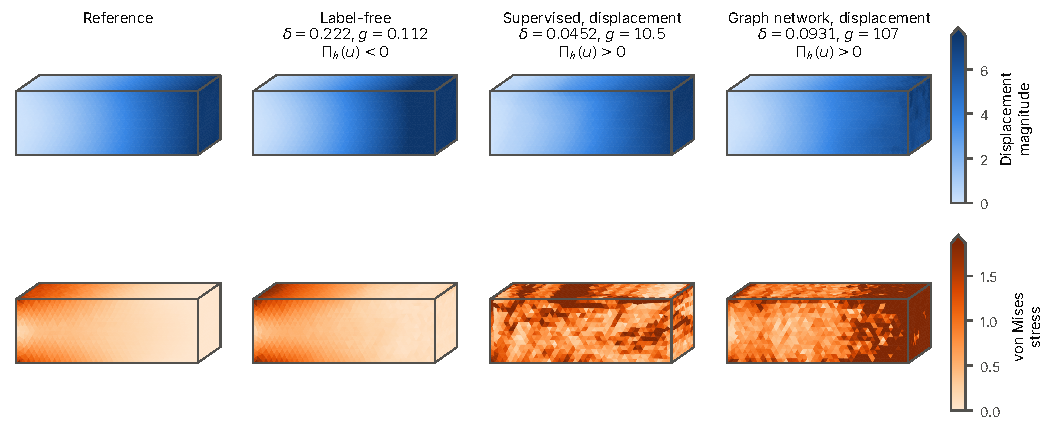
\includegraphics[width=\linewidth]{generated/fig_field_worst.pdf}
\caption{Validation instance No.~\numWorstIndex{}, seed 0, under the \numFigWorstLoad{}:
magnitude of the displacement (top) and von Mises stress (bottom) of the reference solution
and of three networks trained on 1,024 instances, on the three visible faces of the box;
each row has one colour scale, set by the reference, and darker values saturate. Above each
network, its relative displacement error $\delta$ and relative energy gap $g$ on this load
case and the sign of $\Pi_h(u)$, positive when the prediction is further from the solution,
in the energy norm, than the zero field. The instance is the one with the largest relative
energy gap of the displacement-supervised transformer; the selection rules are in
supplementary Section~\SuppRepro{}.}
\label{fig:field-worst}
\end{figure}

\Cref{fig:field-worst} shows the pattern on one instance, No.~\numWorstIndex{} in seed 0.
Averaged over its four load cases, the label-free transformer had the largest displacement
error of the three networks, \numWorstFreeDisp{}, and the most accurate stresses, with a von
Mises error of \numWorstFreeVm{} and a relative energy gap of \numWorstFreeGap{}. The
displacement-supervised transformer and the graph network had displacement errors of
\numWorstLabDisp{} and \numWorstMgnDisp{}, von Mises errors of \numWorstLabVm{} and
\numWorstMgnVm{}, and relative energy gaps of \numWorstLabGap{} and \numWorstMgnGap{}: both
were more accurate in displacement and worse than the zero field in energy. On the load case
shown, the three displacement fields have the shape of the reference, the label-free one
with too large an amplitude: its relative displacement error of \numFigWorstFreeDisp{} falls
to \numFigWorstFreeDispC{} when it is rescaled by $\cstar=\numFigWorstFreeC{}$
(\cref{prop:amp}). The stress fields of the two networks trained on the displacement error
are rough, and more than twice the reference's on \numFigWorstTwiceLab{} and
\numFigWorstTwiceMgn{} of the solid's volume, against \numFigWorstTwiceFree{} for the
label-free transformer; a typical instance, on which their predictions were better than the
zero field, shows the same roughness (supplementary Section~\SuppThree{}). Small
displacement errors rich in stiff modes are what \cref{sec:norm:spectrum} measured, and by
\cref{prop:stress} they are large stress errors.

\subsection{Predictions worse than the zero field}\label{sec:checks:zero}

\begin{figure}[tbp]
\centering
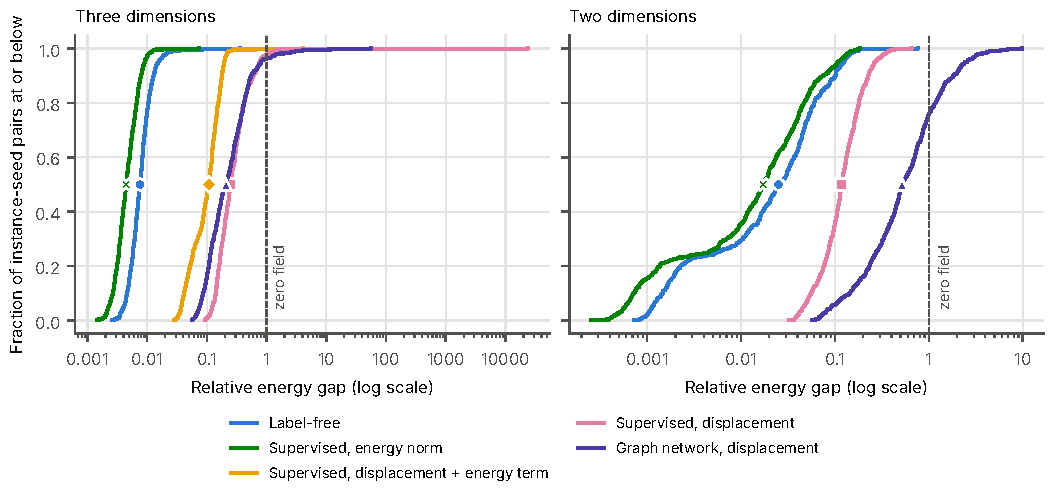
\includegraphics[width=\linewidth]{generated/fig_energy_gap.pdf}
\caption{Distribution of the relative energy gap, averaged over each instance's four load
cases, over the \numThreePairs{} validation instance-seed pairs, networks trained on 1,024
instances, in three dimensions (left) and two (right). Markers show the medians over the
pairs; predictions to the
right of the dashed line are further from the solution, in the energy norm, than the zero
field, on average over their load cases.}
\label{fig:energygap}
\end{figure}

In three dimensions none of the \numThreePairs{} instance-seed predictions of the label-free
or of the energy-norm-supervised transformer had a mean relative energy gap above one
(\cref{fig:energygap}), against \numThreeLabWorse{} of the displacement-supervised
transformer's, \numThreeAncWorse{} of the variant with the energy term and
\numThreeMgnWorse{} of the graph network's; the label-free transformer's median over the
pairs, \numThreeFreeGapMedian{}, was \numThreeMedianRatioMin{} to \numThreeMedianRatioMax{}
times lower than the medians of the networks trained on the displacement error. In two
dimensions \numCmMgnWorse{} of the graph network's predictions had a mean relative energy
gap above one, and none of any transformer's. These counts use the solutions. Load case by
load case, with the test of \cref{cor:zero}, which does not, \numFieldLoadWorseLab{} of the
displacement-supervised transformer's \numFieldLoads{} three-dimensional predictions and
\numFieldLoadWorseMgn{} of the graph network's had a positive energy, and so were worse than
the zero field, against \numThreeFreeLoadWorse{} of the label-free transformer's; in two
dimensions, \numSpecLoadWorseMgn{} of the graph network's \numSpecLoads{} against at most
one of each transformer's. These counts were made after the runs; on the held-out instances
the same test was a pre-registered claim, and it found \numHoldTThreeLab{} and
\numHoldTThreeMgn{} of \numHoldTThreeLoads{} load cases of the two networks trained on the
displacement error in three dimensions, each with a positive energy and no other
(\cref{tab:holdout}). After the rescaling by $\cstar$, none of the three-dimensional
predictions flagged was worse than the zero field, and the rescaling never increased a
relative energy gap.

The check needs only the assembled $K$ and $F$ and applies to any network, however it was
trained, and the rescaling repairs what it flags without a solution (\cref{prop:amp}). It
catches gross failures only: the displacement-supervised transformer's median prediction in
three dimensions, with a relative energy gap of \numThreeLabGapMedian{}, passed it.
